\documentclass[dvipdfmx,a4paper]{jsarticle}
\usepackage{amsmath,amssymb}
\usepackage{amsthm}
\usepackage{bm}
\usepackage[dvipdfmx]{graphicx}
\usepackage{ascmac}
\usepackage{subfigure}
\usepackage{verbatim}
\usepackage{wrapfig}
\usepackage{makeidx}
\usepackage[dvipdfmx]{hyperref}
\usepackage{setspace}
\usepackage{color}
\usepackage{listings}
\usepackage{cleveref}
\usepackage{mathtools}
\usepackage{framed}
\usepackage[textwidth=50zw,lines=46]{geometry}
\usepackage{here}
\usepackage{siunitx}

\usepackage{listings, jlisting, color}
\definecolor{OliveGreen}{rgb}{0.0,0.6,0.0}
\definecolor{Orenge}{rgb}{0.89,0.55,0}
\definecolor{SkyBlue}{rgb}{0.28, 0.28, 0.95}
\lstset{
  language={C++}, % 言語の指定
  basicstyle={\ttfamily},
  identifierstyle={\small},
  commentstyle={\smallitshape},
  keywordstyle={\small\bfseries},
  ndkeywordstyle={\small},
  stringstyle={\small\ttfamily},
  frame={tb},
  breaklines=true,
  columns=[l]{fullflexible},
  numbers=left,
  xrightmargin=0zw,
  xleftmargin=3zw,
  numberstyle={\scriptsize},
  stepnumber=1,
  numbersep=1zw,
  lineskip=-0.5ex,
  keywordstyle={\color{SkyBlue}},     %キーワード(int, ifなど)の書体指定
  commentstyle={\color{OliveGreen}},  %注釈の書体
  stringstyle=\color{Orenge}          %文字列
}

\begin{document}

\title{課題演習C3\quad 最終レポート}
\author{0500-34-0042\quad 大平 達也}
\date{\today}
\maketitle
\section{目的}
系外惑星TOI-1516 bのTransit検出を目標とする。

\section{観測}
京都大学理学部4号館屋上の\SI{40}{cm}望遠鏡を用いて, ノンフィルターでの観測を行った。分かっている, 観測日におけるターゲットの情報は以下の通り:
\begin{description}
  \item[観測日] 2024/11/11
  \item[ingress] 20:00
  \item[degrees] 22:50
  \item[視等級] 10.8 mag
  \item[減光量] 0.016 mag
\end{description}

今回は, 前に観測した天体との兼ね合いで, ingressの途中から観測を始めた。積分時間は10秒, 画像枚数は963枚であった。途中, ターゲット星の再導入のために観測を一時中断したタイミングがあった。

\section{データ処理・結果}
一次処理ののち, 各画像について開口測光を行った。相対測光により, TOI-1516の系の等級を各画像で求め, この時間変化をplotした光度曲線を作成した。これを図\ref{fig:TOI-1516}に示す。図\ref{fig:TOI-1516}の赤い線は, 30点での移動平均を取ることで分散を低減したものである。

これらのデータ処理はすべてPythonで行った。実装の方針としては, 各画像において恒星の位置は大きく変わらないことから, 前の画像のターゲット星, 参照星の物理座標から, 10 pxl以内で最も明るい天体を測光した。視野内で最も明るい天体からのオフセットで, ターゲット星, 参照星の座標を取得する方法も検討したが, 途中で最も明るい天体が画像の外に出てしまっていたことから, この方法は採用しなかった。

最後に, 開口測光のアパーチャー半径は, 半値幅の1.2倍とした。この値は\cite{howell2012}に従った。

\begin{figure}[H]
  \centering
  \includegraphics[width=0.9\textwidth]{./fig/light_curve_TOI1516_with_moving_average.png}
  \caption{TOI-1516の光度曲線}
  \label{fig:TOI-1516}
\end{figure}

\section{議論・考察}
\subsection{参照星の選び方について}
参照星は, 常に視野内に位置し, ターゲット星と同程度の明るさのものを選んだ。また, 測光したのちに, 参照星の等級の時間変化を調べ, 参照星として適切であるかを検証した。

たとえば, 最初に選んだ参照星の等級の時間変化は図\ref{fig:comp}であった。全体として同じようなトレンドではあるが, Comp 4 (紫) のみノイズが大きいように見える。実際, Comp 4が参照星の中で最も暗い星であったことからS/Nが他と比べて小さく, 参照星として選ぶのは適切でないと判断し, 他の参照星を選んだ。これを繰り返すことで, 最終的な参照星を選んだ。最終的な参照星を, 図\ref{fig:finding_chart}に示す。

\begin{figure}[H]
  \centering
  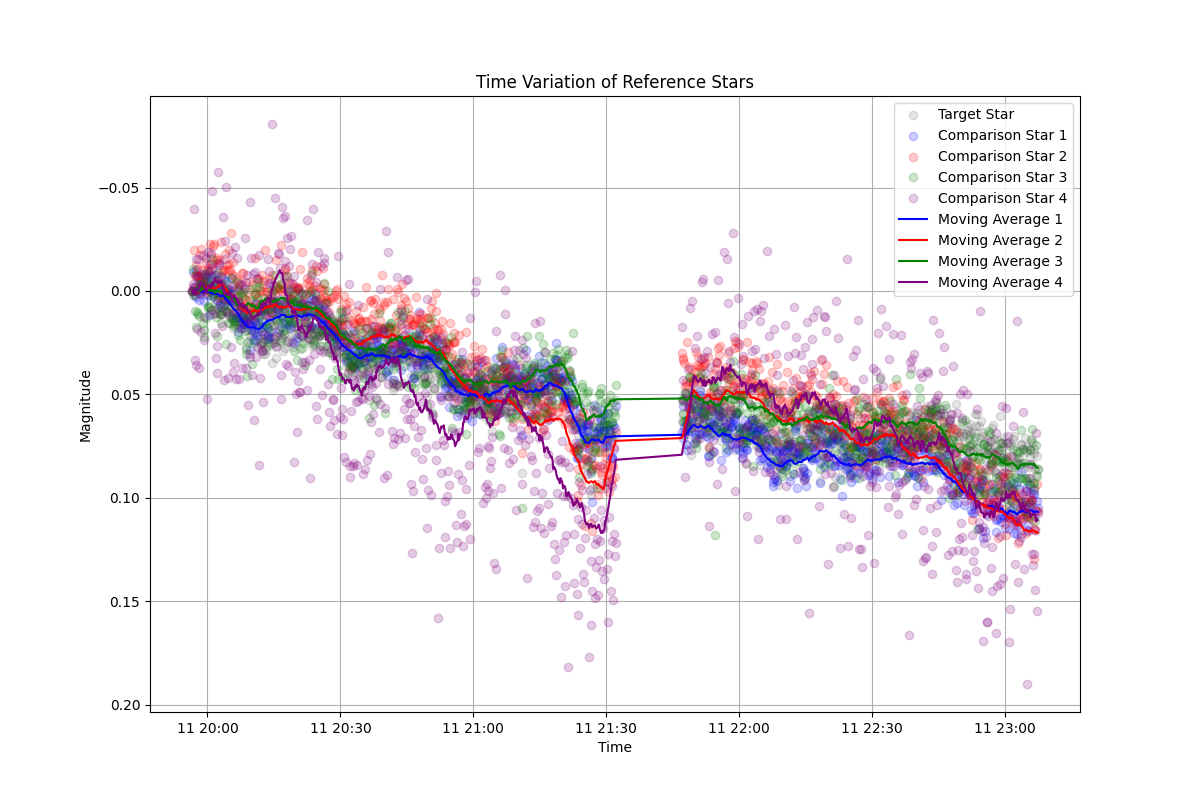
\includegraphics[width=0.9\textwidth]{./fig/light_curve_comp_first.png}
  \caption{参照星の光度曲線}
  \label{fig:comp}
\end{figure}

\begin{figure}[H]
  \centering
  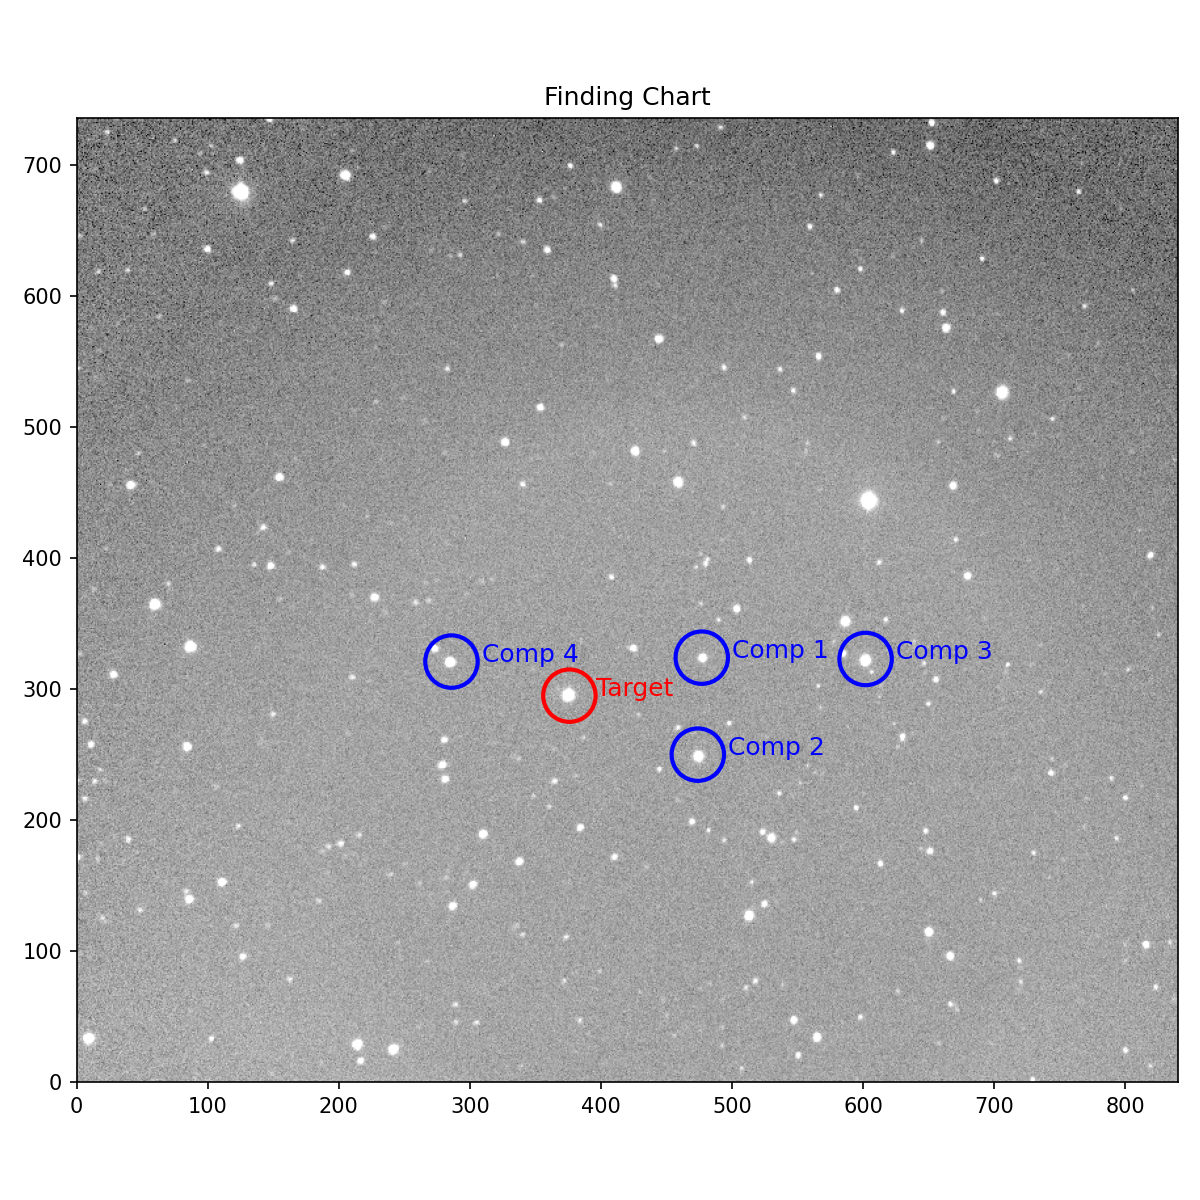
\includegraphics[width=0.65\textwidth]{./fig/finding_chart.png}
  \caption{参照星のfinding chart}
  \label{fig:finding_chart}
\end{figure}

\subsection{参照星のクオリティチェックについて}
最終的な参照星のクオリティチェックは, 参照星の等級の分散を計算することで行った。参照星の等級の分散が小さいほど, 参照星として適切であると考えられる。

具体的には, すべての参照星のフラックスの平均の値を用いて, 各参照星のフラックスを補正した。その後, それぞれの参照星の等級の分散を計算した。最後に, フラックスの変化が1\%を超えるようであれば, フラックスの変化が1\%程度になるよう, 最低限のビンで移動平均を取った。

参照星の等級の分散は表\ref{tab:compstars}の通りであった。これらの値は, トランジットの深さが\SI{0.016}{mag}であることを考えると, 十分に小さい値であると考えられる。

ここで, フラックス変化が$\Delta F/F$のときの等級の変化$\Delta m$は, 
$$\Delta m= -2.5\log(1+\Delta F/F)\simeq -2.5\times \dfrac{1}{\ln 10}\dfrac{\Delta F}{F}\simeq -1.09\dfrac{\Delta F}{F}$$
であるため, フラックスの変化が1\%程度であれば, 等級の変化は約\SI{0.01}{mag}程度である。そのため, 観測データの品質は十分であると考えられる。

\begin{table}[htbp]
  \centering
  \caption{参照星の等級の分散と標準偏差}
  \label{tab:compstars}
  \begin{tabular}{c c c}
  \hline
  Comp & 分散 & 標準偏差 \\
  \hline
  1 & 0.00011 & 0.01028 \\
  2 & 0.00006 & 0.00782 \\
  3 & 0.00005 & 0.00693 \\
  4 & 0.00016 & 0.01249 \\
  \hline
  \end{tabular}
\end{table}

\subsection{トランジットモデルとデータの比較}
これまでの議論により, 観測から品質の良いトランジット光度曲線を作成することができ, トランジットを確認することができた。次に, カタログ値からトランジットモデルを作成し, これらを比較する。恒星系のパラメータの値は, \cite{Kabath2022}に従った。

実装の方針を述べる。トランジットモデルの計算には, batmanというライブラリを用いた。トランジットモデルを計算する際に, トランジット中心時間をユリウス日で与え, 最後にdatetimeに変換した。これにより観測データとトランジットモデルの時間を合わせることができ, トランジットモデルと観測による光度曲線を同一の図にplotすることができた。また, 縦軸は, 観測データから補正したフラックスの, 最後の50点の中央値を1とする相対値を取った。

図\ref{fig:transit_model}に, これによって得られた光度曲線を示す。モデルの曲線が概ねデータの範囲に収まっていることが確認された。

\begin{figure}[H]
  \centering
  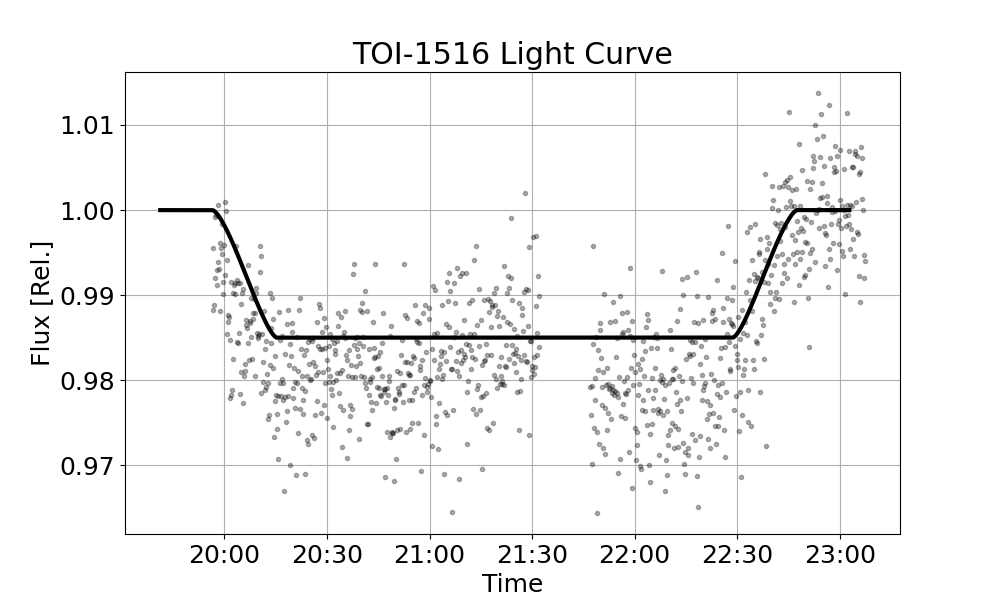
\includegraphics[width=0.9\textwidth]{./fig/light_curve_fit.png}
  \caption{TOI-1516の光度曲線}
  \label{fig:transit_model}
\end{figure}

\begin{thebibliography}{9}
\bibitem{howell2012}
Steve B. Howell, \textit{Handbook of CCD Astronomy}, 2nd ed., Cambridge University Press, 2012.
\bibitem{Kabath2022}
Kabáth, P., Chaturvedi, P., et al.\ 
2022, 
\textit{Monthly Notices of the Royal Astronomical Society}, 
513(4), 5955--5972.
\end{thebibliography}
\end{document}